\documentclass{article}
\usepackage{graphicx} % Required for inserting images
\usepackage{amsmath, amssymb, mathtools, dirtytalk}
\graphicspath{{Images/}}

\setlength{\oddsidemargin}{0in}
\setlength{\textwidth}{6.5in}
\setlength{\topmargin}{-.55in}
\setlength{\textheight}{9in}
\pagestyle{empty}


\title{Optimization HW 6}
\author{Michael Nameika}
\date{March 2023}

\begin{document}

\maketitle

\section*{Section 11.2 Problems}
\textbf{3.} 
Consider the function
\[f(x_1,x_2) = 8x_1^2 + 3x_1x_2 + 7x_2^2 - 25x_1 + 31x_2 - 29\]
Find all stationary points of this function and determine whether they are local minimizers and maximizers. Does this function have a global minimizer or a global maximizer?
\newline\newline
To find all stationary points, we must solve $\nabla f = 0$. Well,
\[\nabla f(x_1,x_2) = \begin{pmatrix*}[r]
    16x_1 + 3x_2 - 25\\
    3x_1 + 14x_2 + 31
\end{pmatrix*}\]
So we wish to solve 
\begin{align*}
    \begin{pmatrix*}[r]
        16 & 3\\
        3 & 14
    \end{pmatrix*}\begin{pmatrix*}
        x_1\\
        x_2
    \end{pmatrix*}
     &= \begin{pmatrix*}
         25\\
         -31
     \end{pmatrix*}
\end{align*}    
From this, we get the solution
\[\begin{pmatrix*}[r]
    x_1\\
    x_2
\end{pmatrix*} = \begin{pmatrix*}[r]
    443/215\\
    -571/215
\end{pmatrix*}\]
Now, to determine if this stationary point is a local min/max, let us inspect the Hessian:
\[\nabla^2f(x_1,x_2) = \begin{pmatrix*}[r]
    16 & 3\\
    3 & 14
\end{pmatrix*}\]
The Hessian is positive definite since in row echelon form we have the pivots are positive, as we can see below:
\[\begin{pmatrix*}
    16 & 3\\
    0 & 215/16
\end{pmatrix*}\]
Since the Hessian is positive definite, we have that this point is a local minimum. Additionally, since $\lim_{x_1 \to \infty} f(x_1,x_2), \lim_{x_2 \to \infty} f(x_1,x_2) = \infty$, our point is the global minimum.
\newline\newline
\textbf{13.} Consider the quadratic function
\[f(x) = \frac{1}{2}x^TQx - c^Tx.\]
\begin{itemize}
    \item[(i)] Write the first-order necessary condition. When does a stationary point exist?
    \newline\newline
    Notice that we may rewrite the problem as 
    \[\frac{1}{2}x^TQx - c^Tx = \frac{1}{2}\sum_{k=1}^n\sum_{i=1}^nq_{ki}x_kx_j - \sum_{i=1}^nc_ix_i\]
    From this, we can see that the only terms that have $x_i$ are 
    \[\left[\frac{1}{2}x^TQx - c^T\right]\bigg|_{i} = \frac{1}{2}q_{ii}x_i^2 + \frac{1}{2}\sum_{\substack{k=1\\k\neq i}}^nq_{ki}x_kx_i + \frac{1}{2}\sum_{\substack{j=1\\j\neq i}}^nq_{ij}x_ix_j - c_ix_i\]
    Taking the partial derivative of the above equation with respect to $x_i$, we find
    \begin{align*}
        &\frac{\partial}{\partial x_i}\left(\frac{1}{2}q_{ii}x_i^2 + \frac{1}{2}\sum_{\substack{k=1\\k\neq i}}^nq_{ki}x_kx_i + \frac{1}{2}\sum_{\substack{j=1\\j\neq i}}^nq_{ij}x_ix_j - c_ix_i\right) =\\
        &= q_{ii}x_i + \frac{1}{2}\sum_{\substack{k=1\\k\neq i}}^nq_{ki}x_k + \frac{1}{2}\sum_{\substack{j=1\\j\neq i}}^nq_{ij}x_j - c_i\\
        &= \frac{1}{2}\sum_{k=1}^nq_{ki}x_k + \frac{1}{2}\sum_{j=1}^nq_{ij}x_j - c_i
    \end{align*}
    From this, we can see
    \begin{align*}
        \nabla f(x) = \frac{1}{2}(Q + Q^T)x - c\\
    \end{align*}
    Then for a stationary point $x_*$ to exist, we require $\nabla f(x_*) = 0$, or equivalently, 
    \begin{align*}
        \nabla f(x_*) &= \frac{1}{2}(Q + Q^T)x_* - c = 0\\
        \frac{1}{2}(Q + Q^T)x_* &= c
    \end{align*}
That is, we need $x_*$ to be the solution to the linear system $1/2(Q + Q^T)x_* = c$.
    
    \item[(ii)] Under what conditions on $Q$ does a local minimizer exist?
    \newline\newline
    From the work in part (i), it is easily shows that 
    \[\nabla^2f(x) = \frac{1}{2}(Q + Q^T)\]
    and so we must have that $Q + Q^T$ is positive semidefinite for a local minimizer to exist.

    \item[(iii)] Under what conditions on $Q$ does $f$ have a stationary point, but no local minima nor maxima?
    \newline\newline
    For $f$ to have a stationary point but no local minima nor maxima, $Q + Q^T$ must be indefinite.
    
\end{itemize}



\section*{Section 11.3 Problems}
\textbf{2.} Use Newton's method to solve
\[\text{minimize} \:\:\:\: f(x) = 5x^5 + 2x^3 - 4x^2 - 3x + 2.\]
Look for a solution in the interval $-2 \leq x \leq 2$. Make sure that you have found a minimum and not a maximum. You may want to experiment with different initial guesses of the solution.
\newline\newline
Implementing Newton's method in MATLAB, with the initial guess $x_0 = 0$, we arrive at the stationary point $x_* \approx -0.2899$, which, as we can see from the images below, is a local maximum since $f''(x) < 0$:
\begin{center}
    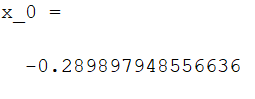
\includegraphics[scale = 0.9]{initGuess_0}
    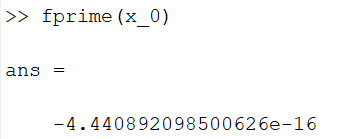
\includegraphics[scale = 0.9]{fprime_init_0}
    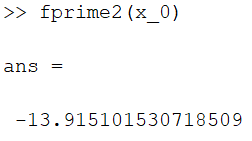
\includegraphics[scale = 0.9]{fprime2_0}
    \newline\newline\newline
\end{center}
Since we are searching for a minimum, this stationary point is not optimal. Trying the initial guess $x_0 = 1$, we arrive at the stationary point $x_* \approx 0.6899$, which, from the images below, is a local minimum of $f$.
\newline\newline
\begin{center}
    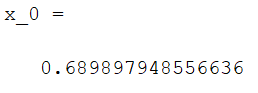
\includegraphics[scale = 0.9]{initGuess_1}
    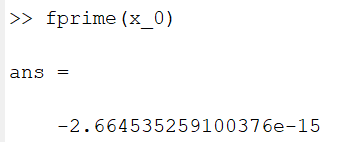
\includegraphics[scale = 0.9]{fprime_init_1}
    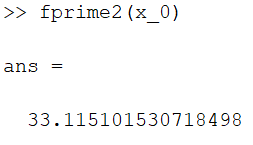
\includegraphics[scale = 0.9]{fprime2_1}
    \newline\newline\newline
\end{center}
The corresponding value of $f$ is 
\[f(x_*) \approx -0.5354\]
\newline\newline\newline
\textbf{3.} Use Newton's method to solve
\[\text{minimize}\:\:\:\: f(x_1,x_2) = 5x_1^4 + 6x_2^4 - 6x_1^2 + 2x_1x_2 + 5x_2^2 + 15x_1 - 7x_2 + 13.\]
Use the initial guess $(1,1)^T$. Make sure that you have found a minimum and not a maximum.
\newline\newline
Implementing Newton's method for this problem in MATLAB, with the initial guess of $(1,1)^T$, we find the following stationary point:
\newline
\[x_* \approx \begin{pmatrix*}[r]
    -1.42\\
    0.5434
\end{pmatrix*}\]
\newline
And, from the images below, we can see that $\nabla^2f(x_*)$ is positive definite (since the eigenvalues of $\nabla^2f(x_*)$ are strictly positive), so $x_*$ corresponds to a local minimum.
\begin{center}
    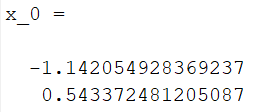
\includegraphics[scale = 0.9]{prob3_3_min}
    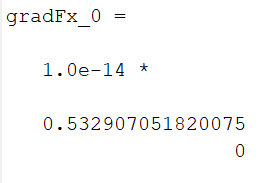
\includegraphics[scale = 0.9]{prob3_3_grad}
    \newline\newline\newline
    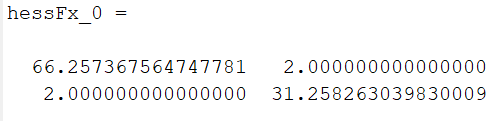
\includegraphics[scale = 0.9]{prob3_3_hess}
    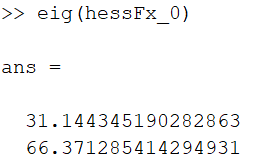
\includegraphics[scale = 0.9]{prob3_3_hesseig}
    \newline\newline
\end{center}
The corresponding value of $f$ is
\[f(x_*) \approx -6.496\]
\newline\newline
\textbf{7.} The purpose of this exercise is to prove Theorem 11.2. Assume that the assumptions of the theorem are satisfied.
\begin{itemize}
    \item[(i)] Prove that
    \[x_{k+1} - x_* = \nabla^2f(x_k)^{-1}[\nabla^2f(x_k)(x_k - x_*) - (\nabla f(x_k) - \nabla f(x_*))].\]
    \newline\newline\newline
    Proof: Assume that $\nabla^2f(x)$ is Lipschitz continuous on an open convex set S and $x_* \in S$ is a stationary point of $f(x)$ From Newton's method, we have that
    \newline
    \[x_{k+1} = x_k - \left[\nabla^2f(x_k)\right]^{-1}\nabla f(x_k)\]
    \newline
    Subtracting $x_*$ from each side, we obtain
    \newline
    \[x_{k+1} - x_* = x_k - x_* - \left[\nabla^2f(x_k)\right]^{-1}\nabla f(x_k)\]
    \newline
    and so we may rewrite the above equation as
    \newline
    \[x_{k+1} - x_* = \left[\nabla^2f(x_k)\right]^{-1}\left(\nabla^2f(x_k)(x_k - x_*) - \nabla f(x_k)\right)\]
    \newline
    since $x_*$ is a stationary point, we have that $\nabla f(x_*) = 0$ and so we can add $\nabla f(x_*)$ into the above equation to obtain
    \newline
    \[x_{k+1} - x_* = \left[\nabla^2f(x_k)\right]^{-1}\left(\nabla^2f(x_k)(x_k - x_*) - (\nabla f(x_k) - \nabla f(x_*))\right)\]
    \newline
    Which is what we sought to show.
    \item[(iii)] Prove that for large enough $k$,
    \[\|x_{k+1} - x_*\| \leq L\left\|\nabla^2f(x_k)^{-1}\right\|\|x_k - x_*\|^2.\]
    and from here prove the results of the theorem.
    \newline\newline
    Proof: Suppose $\nabla^2f(x)$ is Lipschitz continuous on an open convex set $S$ and begin by noticing that
    \begin{align*}
        \nabla f(x_k) &= \nabla f(x_* + (x_k - x_*))\\
    \end{align*}
    And so by Taylor's theorem,
    \begin{align*}
        \nabla f(x_* + x_k - x_*) &= \nabla f(x_*) + \nabla^2f(\xi)(x_k - x_*)\\
    \end{align*}
    Where $R$ is the remainder term. Using this in combination with our result from part (i), we have the following:
    \begin{align*}
        x_{k+1} - x_* &= \left[\nabla^2f(x_k)\right]^{-1}\left(\nabla^2f(x_k)(x_k - x_*) - (\nabla f(x_k) - \nabla f(x_*))\right) \\
        &= \left[\nabla^2f(x_k)\right]^{-1}\left(\nabla^2f(x_k)(x_k - x_*) - (\nabla f(x_*) + \nabla^2f(\xi)(x_k - x_*) - \nabla f(x_*))\right)\\
        &= \left[\nabla^2f(x_k)\right]^{-1}\left((\nabla^2f(x_k) - \nabla^2f(\xi))(x_k - x_*)\right)\\
    \end{align*}
    and so
    \begin{align*}
        \|x_{k+1} - x_*\| &= \left\|\left[\nabla^2f(x_k)\right]^{-1}\left((\nabla^2f(x_k) - \nabla^2f(\xi))(x_k - x_*)\right)\right\|\\
        &\leq \left\|\left[\nabla^2f(x_k)\right]^{-1}\right\|\left\|\left(\nabla^2f(x_k) - \nabla^2f(\xi)\right)\right\|\left\|x_k - x_*\right\|\\
        &\leq \left\|\left[\nabla^2f(x_k)\right]^{-1}\right\|\left\|x_k - \xi\right\|\left\|x_k - x_*\right\|\\
    \end{align*}
    Since $\xi \in (x_k, x_*)$ or $\xi \in (x_*, x_k)$, $\|x_k - \xi\| \leq \|x_k - x_*\|$ so
    \begin{align*}
        \|x_{k+1} - x_*\| &\leq L\left\|\left[\nabla^2f(x_k)\right]^{-1}\right\|\|x_k - x_*\|^2\\
    \end{align*}
    Which is what we sought to show.
    \newline\newline
    Now we must prove the main result of Theorem 11.2: that $\{x_k\}$ converges to $x_*$ quadratically. 
    \newline
    Proof: Let $f(x)$ be defined on an open convex set $S$ be such that $\nabla^2f(x)$ is positive definite and Lipschitz continuous and consider the sequence $\{x_k\}$ generated by
    \[x_{k+1} = x_k - \left[\nabla^2f(x_k)\right]^{-1}\nabla f(x_k)\]
    and further assume that $x_*$ is a minimizer of $f$. If $\|x_0 - x_*\|$ is sufficiently small, we wish to show that $\{x_k\}$ converges to $x_*$ quadratically. That is, we wish to show
    \[\lim_{k \to \infty} \frac{\|x_{k+1} - x_*\|}{\|x_k - x_*\|^2} = C < \infty\]
    Well from the result of part (iii) above, we have
    \begin{align*}
        \lim_{k \to \infty}\frac{\|x_{k+1} - x_*\|}{\|x_k - x_*\|^2} &\leq \lim_{k \to \infty}\frac{L\left\|\nabla^2f(x_k)^{-1}\right\|\|x_k - x_*\|^2}{\|x_k - x_*\|^2}\\
        &= \lim_{k \to \infty} L\left\|\nabla^2f(x_k)^{-1}\right\|\\
        &= L\left\|\nabla^2f(x_*)^{-1}\right\|
    \end{align*}
    And so we have $\frac{\|x_{k+1} - x_*\|}{\|x_k - x_*\|}$ converges, and by definition, $\{x_k\}$ converges to $x_*$ quadratically.
    
\end{itemize}
\textbf{8.} Let $\{x_k\}$ be a sequence that converges superlinearly to $x_*$. Prove that
\[\lim_{k \to \infty} \frac{\|x_{k+1} - x_k\|}{\|x_k - x_*\|} = 1\]
\newline\newline\newline
Proof: Let $\{x_k\}$ be a sequence that converges superlinearly to $x_*$. That is,
\newline
\[\lim_{k \to \infty} \frac{\|x_{k+1} - x_*\|}{\|x_k - x_*\|} = 0\]
\newline
We wish to show
\newline
\[\lim_{k \to \infty} \frac{\|x_{k+1} - x_k\|}{\|x_k - x_*\|} = 1\]
\newline
Well, notice, by the triangle inequality
\begin{align*}
    \|x_{k+1} - x_k\| &= \|x_{k+1} - x_* + x_* - x_k\| \leq \|x_{k+1} - x_k\| + \|x_* - x_k\| \\
    &= \|x_{k+1} - x_k\| + \|x_k - x_*\| \\
\end{align*}
By the reverse triangle inequality, we have
\begin{align*}
    \|x_{k+1} - x_k\| &= \|x_{k+1} - x_* + x_* - x_k\| \\
    &= \|x_{k+1} - x_* - (x_k - x_*)\| \\
    &\geq \bigg|\|x_{k+1} - x_*\| - \|x_k - x_*\| \bigg|
\end{align*}
From this, we have
\[\lim_{k \to \infty} \frac{\bigg|\|x_{k+1} - x_*\| - \|x_k - x_*\|\bigg| }{\|x_k - x_*\|} \leq  \lim_{k \to \infty} \frac{\|x_{k+1} - x_k\|}{\|x_k - x_*\|} \leq \lim_{k \to \infty} \frac{\|x_{k+1} - x_*\| + \|x_k - x_*\|}{\|x_k - x_*\|}\]
\newline
Evaluating the lower and upper bound limits, we find
\begin{align*}
    \lim_{k \to \infty} \frac{\bigg| \|x_{k+1} - x_*\| - \|x_k - x_*\| \bigg| }{\|x_k - x_*\|} &= \bigg| \lim_{k \to \infty} \frac{\|x_{k+1} - x_*\|}{\|x_k - x_*\|} - \lim_{k \to \infty} \frac{\|x_k - x_*\|}{\|x_k - x_*\|} \bigg| \\
    &= \bigg| 0 - 1 \bigg| \\
    &= 1
\end{align*}
and
\begin{align*}
    \lim_{k \to \infty} \frac{\|x_{k+1} - x_*\| + \|x_k - x_*\|}{\|x_k - x_*\|} &= \lim_{k \to \infty} \frac{\|x_{k+1} - x_*\|}{\|x_k - x_*\|} + \lim_{k \to \infty} \frac{\|x_k - x_*\|}{\|x_k - x_*\|}\\
    &= 0 + 1\\
    &= 1
\end{align*}
Then we have
\newline
\[1 \leq \lim_{k \to \infty} \frac{\|x_{k+1} - x_k\|}{\|x_k - x_*\|} \leq 1\]
\newline
and by the squeeze theorem, we have
\newline
\[\lim_{k \to \infty} \frac{\|x_{k+1} - x_k\|}{\|x_k - x_*\|} = 1\]
\newline
which is what we sought to show.
\newline\newline\newline
\textbf{9.} Let $f$ be a real-valued function of $n$ variables and assume that $f$, $\nabla f$, and $\nabla^2f$ are continuous. Suppose that $\nabla^2f(\bar{x})$ is nonsingular for some point $\bar{x}$. Prove that there exists constants $\epsilon > 0$ and $\beta > \alpha > 0$ such that
\[\alpha\|x - \bar{x}\| \leq \|\nabla f(x) - \nabla f(\bar{x})\| \leq \beta \|x - \bar{x}\|\]
for all $x$ satisfying $\|x - \bar{x}\| \leq \epsilon$.
\newline\newline\newline
Proof: Let $f: \mathbb{R}^n \to \mathbb{R}$ and suppose $f,\nabla f$, and $\nabla^2f$ are continuous and suppose $\nabla^2f(\bar{x})$ is nonsingular for some $\bar{x}$. Further suppose that $\|x - \bar{x}\| \leq \epsilon$ for some $\epsilon > 0$. Notice that
\[\nabla f(x) = \nabla f(x - \bar{x} + \bar{x})\]
and by Taylor's theorem, we have
\begin{align*}
    \nabla f(x) &= \nabla f(\bar{x}) + (x - \bar{x})^T\nabla^2f(\xi)\\
    \nabla f(x) - \nabla f(\bar{x}) &= (x - \bar{x})^T\nabla^2f(\xi)\\
    \|\nabla f(x) - \nabla f(\bar{x})\| &= \|\nabla^2f(\xi)^T(x - \bar{x})\| \\
    &\leq \|\nabla^2f(\xi)\|\|(x - \bar{x})\|
\end{align*}
Let $\beta = \|\nabla^2f(\xi)\| > 0$. Now we have
\[\|\nabla f(x) - \nabla f(\bar{x})\| \leq \beta \|x - \bar{x}\|\]
Additionally, from above,
\begin{align*}
    \nabla f(x) &= \nabla f(\bar{x}) + \nabla^2f(\xi)(x - \bar{x})^T\\
    \nabla f(x) - \nabla f(\bar{x}) &= \nabla^2(x)(x - \bar{x})^T\\
    \nabla^2f(x)^{-1}(\nabla f(x) - \nabla f(\bar{x})) &= (x - \bar{x})^T\\
    \|\nabla^2f(x)^{-1}(\nabla f(x) - \nabla f(\bar{x}))\| &= \|x - \bar{x}\|
\end{align*}
Then we have 
\begin{align*}
    \|x - \bar{x}\| &\leq \|\nabla f(x) - \nabla f(\bar{x})\|\|\nabla^2f(x)^{-1}\| \\
    \frac{1}{\|\nabla^2f(x)^{-1}\|} \|x - \bar{x}\| &\leq \|\nabla f(x) - \nabla f(\bar{x})\| \\
\end{align*}
Let $\alpha = \frac{1}{\|\nabla^2f(x)^{-1}\|} > 0$. Then we have
\[\alpha \|x - \bar{x}\| \leq \|\nabla f(x) - \nabla f(\bar{x})\| \leq \beta\|x - \bar{x}\|\]

\section*{Section 11.4 Problems}
\textbf{1.} Find a diagonal matrix $E$ so that $A + E = LDL^T$ where 
\[A = \begin{pmatrix}
    1 & 4 & 3\\
    4 & 2 & 5\\
    3 & 5 & 3
\end{pmatrix}\]
\newline
Notice that $a_{11} = 1 > 0$ in this (initial) stage, so we'll leave it alone. Now pivot the first column with the following operations:
\begin{align*}
    &R_2 - 4R_1 \to R_2\\
    &R_3 - 3R_1 \to R_3
\end{align*}
Then $A$ becomes
\[\begin{pmatrix*}[r]
    1 & 4 & 3\\
    0 & -14 & -7\\
    0 & -7 & -6
\end{pmatrix*}\]
Replace $a_{22}$ in this stage with $7$. That is, add 21 to $a_{22}$. Then pivoting the second column, by adding row two to the third row, $A$ becomes
\[\begin{pmatrix*}[r]
    1 & 4 & 3\\
    0 & 7 & -7\\
    0 & 0 & -13
\end{pmatrix*}\]
Now replace $a_{33}$ in this stage with 1. That is, add 14 to $a_{33}$. Then we have 
\[E = \begin{pmatrix}
    0 & 0 & 0\\
    0 & 21 & 0\\
    0 & 0 & 14
\end{pmatrix}\]
Finally, we have
\[A + E = LDL^T\]
with
\[LDL^T = \begin{pmatrix*}[r]
    1 & 0 & 0\\
    4 & 1 & 0\\
    3 & -1 & 1
\end{pmatrix*}\begin{pmatrix}
    1 & 0 & 0\\
    0 & 7 & 0\\
    0 & 0 & 1
\end{pmatrix}\begin{pmatrix*}[r]
    1 & 4 & 3\\
    0 & 1 & -1\\
    0 & 0 & 1
\end{pmatrix*}\]

\end{document}
